
\section{Comparative Analysis of Models}

In this chapter, we explain the performance of different models that we used in our research with the help of graphs, tables, etc

\subsection{Pretrained Model Accuracy and Loss Comparison After Transfer Learning}
\begin{figure}
    \centering
    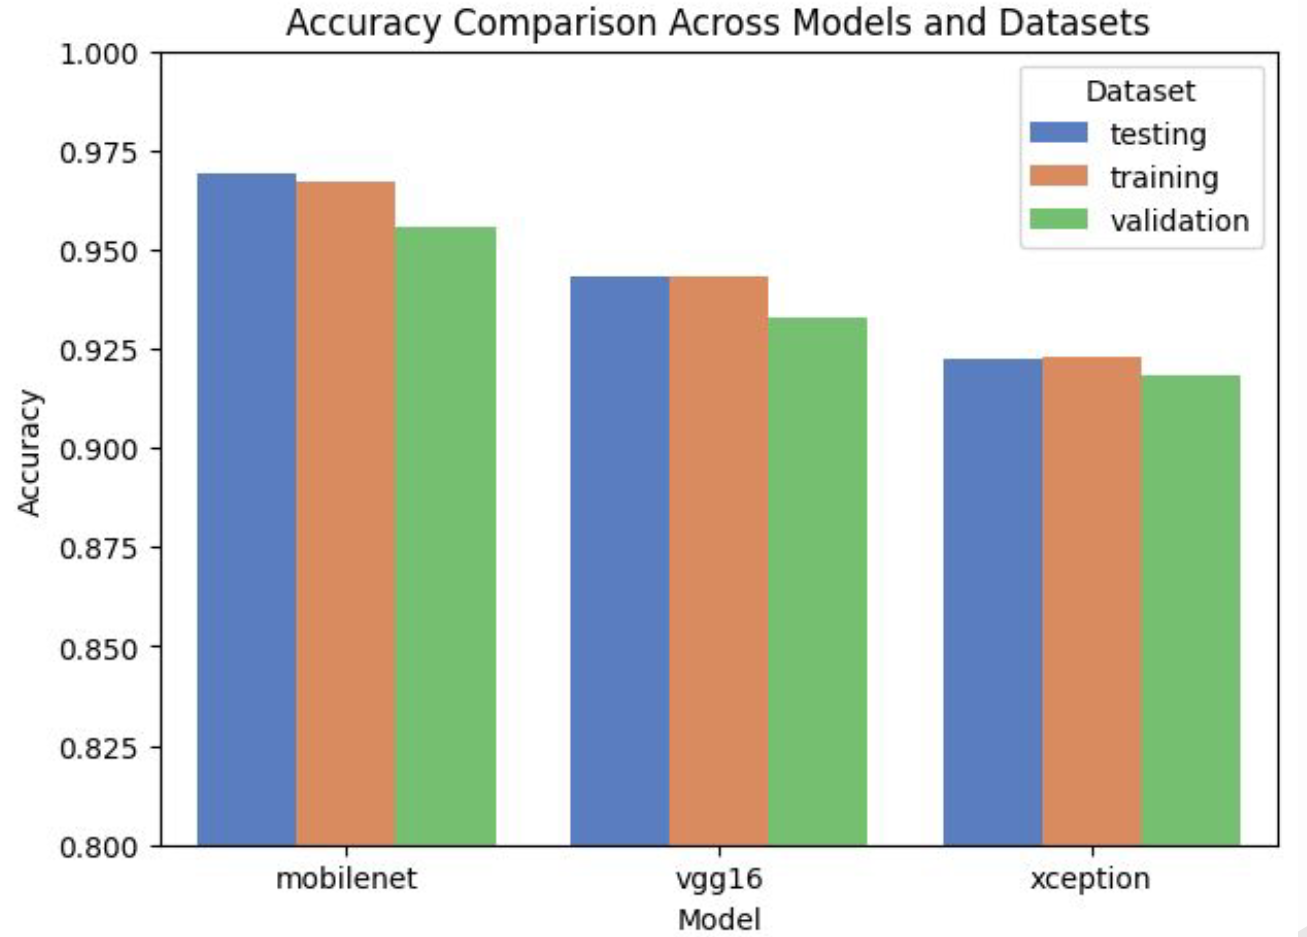
\includegraphics[width=0.75\linewidth]{graphics//chapter6/transfer learning acc.png}
    \caption{Pretrained Model Accuracy After Transfer Learning}
    \label{fig:acc-tf}
\end{figure}

\begin{figure}
    \centering
    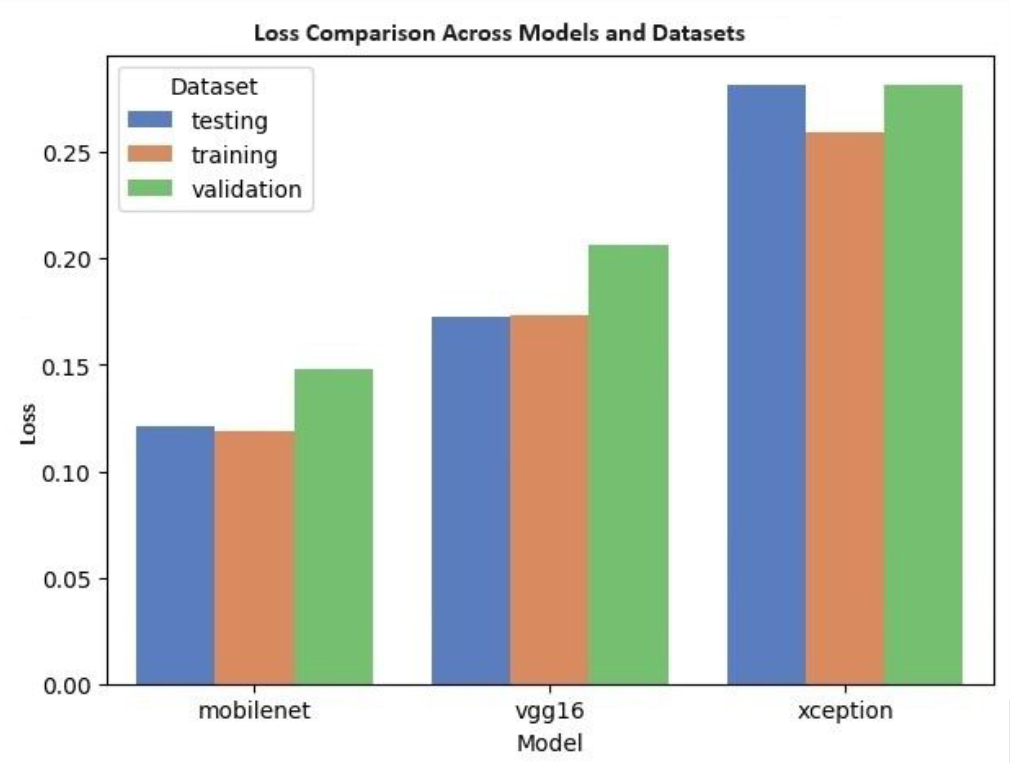
\includegraphics[width=0.75\linewidth]{graphics//chapter6/model loss transfer learning.png}
    \caption{Pretrained Model Loss After Transfer Learning}
    \label{fig:loss-tf}
\end{figure}

After performing transfer learning of our pretrained Convnet models, we observe that MobileNetV2 outperforms all other models with an accuracy of\textbf{\textit{ (0.9670, 0.95589, 0.9693)}} on training, validation and testing datasets, respectively. But, the performance difference between the models is very low, they all perform very well with very little difference. \par\vspace{1em}
As we have already mentioned in methodology section \ref{Transfer-learning-section}, that in transfer learning we are not touching any weights of the base model only the last FCN layer is trained, So, we can inferred from this observation that MobileNetV2 is an excellent feature extractor for generally all classes, even for narrow domain. This is the reason, why we used MobileNetV2 as an feature extractor in combination with other traditional classifeir instead of other convnet model (eg: VGG16, Xception) 
\par\vspace{1em}

% \FloatBarrier


\subsection{Pretrained Model Accuracy and Loss Comparison After Fine Tuning}
\begin{figure}
    \centering
    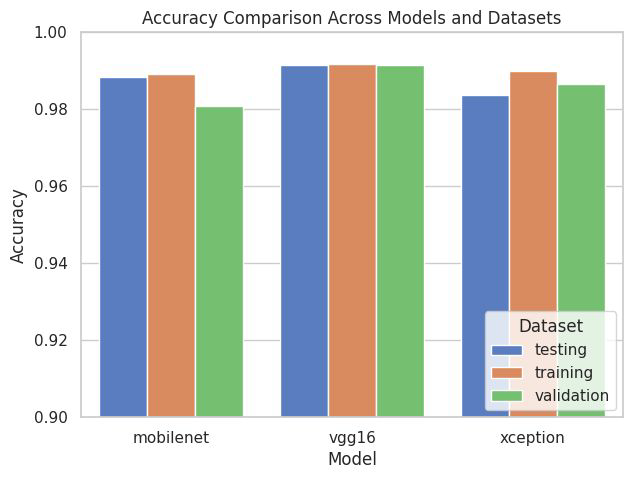
\includegraphics[width=0.75\linewidth]{graphics//chapter6/pretrained acc after fine tuning.png}
    \caption{Pretrained Model Accuracy After Fine Tuning}
    \label{fig:acc-ft}
\end{figure}

\begin{figure}
    \centering
    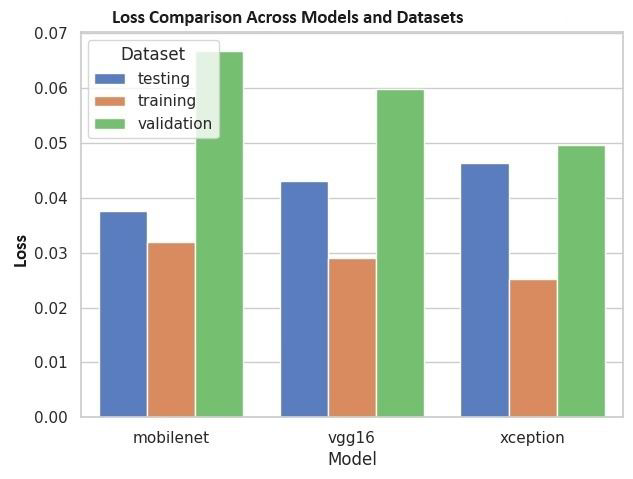
\includegraphics[width=0.75\linewidth]{graphics//chapter6/model loss after fine tuning.png}
    \caption{Pretrained Model Loss after Fine Tuning}
    \label{fig:loss-ft}
\end{figure}

When performing fine tuning the models, we observe that  VGG16 base model, outperform  other models even MobileNet. However, the difference in model accuracy with these 3 models, is very low, they only differ by about 1\% in their accuracy. So, we can say they perform in par with each other.\par\vspace{1em}

% \FloatBarrier

\subsection{Model Comparison with our CNN10L Model}
When comparing our CNN10L model (model that we trained from scratch), against the three pre-trained deep learning models: MobileNetV2, VGG16, and Xception, we observed that the CNN10L model perform badly in all classification evaluation metrics but not by much. In term of accuracy metric, CNN10L get (0.9648, 0.9681, 0.952107) in comparison to the best performing model  (0.9917, 0.9913, 0.9913) in training, validation and testing datasets, respectively.
\par\vspace{1em}
\begin{figure}
    \centering
    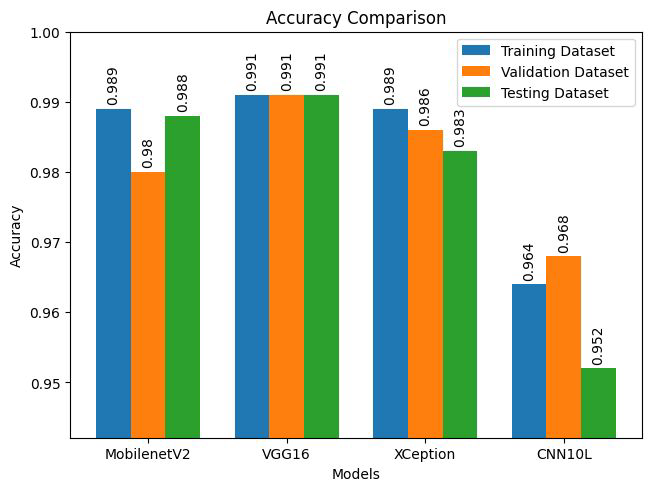
\includegraphics[width=1\linewidth]{graphics//chapter6/nn model acc.png}
    \caption{Neural Network Model Accuracy Comparisons}
    \label{fig:nn-acc}
\end{figure}

\begin{figure}
    \centering
    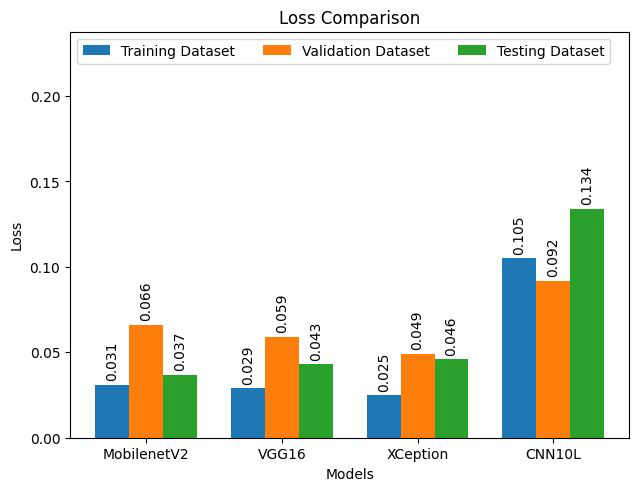
\includegraphics[width=1\linewidth]{graphics//chapter6/nn loss comparison.png}
    \caption{Neural Network Model Loss Comparisons}
    \label{fig:nn-loss}
\end{figure}

% \FloatBarrier

\subsection{Comparison of all model using different evaluation metrics}
 In this section, we perform comparison of all the models that we used.
 \par\vspace{1em}
 The highest accuracy model from our comparison was VGG16, which is a pretrained model, with 0.99 accuracy. Our custom model got an accuracy rating of 0.95. The least accurate model was a traditional model utilizing RandomForest yielding an accuracy rating of 0.84 in accuracy of testing dataset.
 \par\vspace{1em}
 
After these rigorous comparisons between the various models using different evaluation matrices, the consensus is that pre-trained deep learning models have a noticeable increase in performance and accuracy, over model trained from scratch and  traditional models. Pre-trained models also have some increase in performance and accuracy over our custom trained model, CNN10L.\par \vspace{1em}

From this observation, we inferred that, the knowledge that is learned by pretrained model from large datasets like ImageNet is actually helpful in performing classification in narrow domain tasks as our scratch model, CNN10L is easily outperform by the 3 pretrained base model in term of accuracy, precision, recall and F1-score.
\par\vspace{1em}
Among traditional classifier models, we observe that SVM and XGBoost perform the best and Random Forest is the worst-performing one. Even though CNN10L outperform  traditional classifier, the difference in metrics score is very small (3\% difference in accuracy metric) with the best performing traditional classifier model (SVM and XGBoost). So, we can say that these classical models are in par with neural network models and we should not completely ignore them. 
\par\vspace{1em}



\newgeometry{left=1cm,right=1cm}
\begin{table}[h]
    \centering
    \resizebox{\textwidth}{!}{%
    \begin{tabular}{lccccccccccccc}
        \toprule
        \textbf{Model} & \textbf{Measure} & \multicolumn{11}{c}{Classes} & \textbf{Accuracy}\\
         &  & \textbf{0} & \textbf{1} & \textbf{2} & \textbf{3} & \textbf{4} & \textbf{5} & \textbf{6} & \textbf{7} & \textbf{8} & \textbf{9} & \textbf{10}\\
         
        \midrule
        
        \textbf{MobileNetV2} & \textbf{Precision} & \textbf{1.00} & \textbf{1.00} & \textbf{0.96} & \textbf{1.00} & \textbf{1.00} & \textbf{1.00} & \textbf{1.00} & \textbf{1.00} & \textbf{1.00} & \textbf{1.00} & \textbf{0.86} & \textbf{}\\
        \textbf{} & \textbf{Recall} & \textbf{1.00} & \textbf{1.00} & \textbf{0.96} & \textbf{1.00} & \textbf{1.00} & \textbf{1.00} & \textbf{1.00} & \textbf{0.88} & \textbf{1.00} & \textbf{1.00} & \textbf{0.99} & \textbf{}\\
        \textbf{} & \textbf{F1-Score} & \textbf{1.00} & \textbf{1.00} & \textbf{0.98} & \textbf{1.00} & \textbf{1.00} & \textbf{1.00} & \textbf{1.00} & \textbf{0.88} & \textbf{1.00} & \textbf{1.00} & \textbf{0.92} & \textbf{0.99}\\
        \textbf{} & \textbf{Support} & \textbf{63} & \textbf{62} & \textbf{26} & \textbf{164} & \textbf{150} & \textbf{85} & \textbf{105} & \textbf{65} & \textbf{119} & \textbf{116} & \textbf{85} & \textbf{1040}\\
        
        \midrule
        
        \textbf{VGG16} & \textbf{Precision} & \textbf{1.00} & \textbf{1.00} & \textbf{1.00} & \textbf{1.00} & \textbf{1.00} & \textbf{1.00} & \textbf{1.00} & \textbf{0.71} & \textbf{1.00} & \textbf{1.00} & \textbf{1.00} & \textbf{}\\
        \textbf{} & \textbf{Recall} & \textbf{1.00} & \textbf{1.00} & \textbf{1.00} & \textbf{1.00} & \textbf{1.00} & \textbf{1.00} & \textbf{1.00} & \textbf{1.00} & \textbf{1.00} & \textbf{1.00} & \textbf{0.87} & \textbf{}\\
        \textbf{} & \textbf{F1-Score} & \textbf{1.00} & \textbf{1.00} & \textbf{1.00} & \textbf{1.00} & \textbf{1.00} & \textbf{1.00} & \textbf{1.00} & \textbf{0.83} & \textbf{1.00} & \textbf{1.00} & \textbf{0.93} & \textbf{0.99}\\
        \textbf{} & \textbf{Support} & \textbf{63} & \textbf{62} & \textbf{27} & \textbf{164} & \textbf{150} & \textbf{85} & \textbf{105} & \textbf{36} & \textbf{119} & \textbf{116} & \textbf{113} & \textbf{1040}\\
        
        \midrule
        
        \textbf{Xception} & \textbf{Precision} & \textbf{0.98} & \textbf{1.00} & \textbf{1.00} & \textbf{1.00} & \textbf{0.98} & \textbf{0.99} & \textbf{0.97} & \textbf{0.88} & \textbf{0.99} & \textbf{1.00} & \textbf{0.97} & \textbf{}\\
        \textbf{} & \textbf{Recall} & \textbf{0.98} & \textbf{1.00} & \textbf{0.93} & \textbf{0.97} & \textbf{1.00} & \textbf{1.00} & \textbf{1.00} & \textbf{0.94} & \textbf{1.00} & \textbf{1.00} & \textbf{0.93} & \textbf{}\\
        \textbf{} & \textbf{F1-Score} & \textbf{0.98} & \textbf{1.00} & \textbf{0.96} & \textbf{0.98} & \textbf{0.99} & \textbf{0.99} & \textbf{0.99} & \textbf{0.91} & \textbf{1.00} & \textbf{1.00} & \textbf{0.95} & \textbf{0.98}\\
        \textbf{} & \textbf{Support} & \textbf{63} & \textbf{62} & \textbf{29} & \textbf{169} & \textbf{147} & \textbf{84} & \textbf{102} & \textbf{48} & \textbf{118} & \textbf{116} & \textbf{102} & \textbf{1040}\\

        \midrule

        \textbf{CNN10L} & \textbf{Precision} & \textbf{0.90} & \textbf{0.97} & \textbf{1.00} & \textbf{0.98} & \textbf{0.94} & \textbf{1.00} & \textbf{0.98} & \textbf{0.80} & \textbf{1.00} & \textbf{0.86} & \textbf{1.00} & \textbf{}\\
        \textbf{} & \textbf{Recall} & \textbf{0.89} & \textbf{0.98} & \textbf{0.92} & \textbf{0.98} & \textbf{0.97} & \textbf{0.96} & \textbf{0.98} & \textbf{0.77} & \textbf{1.00} & \textbf{0.89} & \textbf{0.99} & \textbf{}\\
        \textbf{} & \textbf{F1-Score} & \textbf{0.89} & \textbf{0.98} & \textbf{0.96} & \textbf{0.98} & \textbf{0.95} & \textbf{0.98} & \textbf{0.98} & \textbf{0.78} & \textbf{1.00} & \textbf{0.88} & \textbf{1.00} & \textbf{0.95}\\
        \textbf{} & \textbf{Support} & \textbf{81} & \textbf{62} & \textbf{25} & \textbf{166} & \textbf{137} & \textbf{111} & \textbf{82} & \textbf{56} & \textbf{114} & \textbf{94} & \textbf{116} & \textbf{1044}\\

        \midrule

        \textbf{SVM} & \textbf{Precision} & \textbf{0.96} & \textbf{0.98} & \textbf{0.98} & \textbf{0.91} & \textbf{0.92} & \textbf{0.92} & \textbf{0.84} & \textbf{0.92} & \textbf{0.96} & \textbf{0.87} & \textbf{0.88} & \textbf{}\\
        \textbf{} & \textbf{Recall} & \textbf{0.98} & \textbf{0.99} & \textbf{0.95} & \textbf{0.96} & \textbf{0.73} & \textbf{0.98} & \textbf{0.63} & \textbf{0.94} & \textbf{0.83} & \textbf{0.92} & \textbf{0.93} & \textbf{}\\
        \textbf{} & \textbf{F1-Score} & \textbf{0.97} & \textbf{0.99} & \textbf{0.96} & \textbf{0.93} & \textbf{0.81} & \textbf{0.95} & \textbf{0.72} & \textbf{0.93} & \textbf{0.89} & \textbf{0.89} & \textbf{0.90} & \textbf{0.93}\\
        \textbf{} & \textbf{Support} & \textbf{99} & \textbf{147} & \textbf{100} & \textbf{100} & \textbf{15} & \textbf{212} & \textbf{100} & \textbf{190} & \textbf{95} & \textbf{177} & \textbf{167} & \textbf{1402}\\

        \midrule

        \textbf{XGBoost} & \textbf{Precision} & \textbf{0.96} & \textbf{0.98} & \textbf{0.98} & \textbf{0.90} & \textbf{0.92} & \textbf{0.92} & \textbf{0.84} & \textbf{0.92} & \textbf{0.96} & \textbf{0.87} & \textbf{0.88} & \textbf{}\\
        \textbf{} & \textbf{Recall} & \textbf{0.98} & \textbf{0.99} & \textbf{0.95} & \textbf{0.96} & \textbf{0.73} & \textbf{0.98} & \textbf{0.63} & \textbf{0.94} & \textbf{0.83} & \textbf{0.92} & \textbf{0.93} & \textbf{}\\
        \textbf{} & \textbf{F1-Score} & \textbf{0.97} & \textbf{0.99} & \textbf{0.96} & \textbf{0.93} & \textbf{0.81} & \textbf{0.95} & \textbf{0.72} & \textbf{0.93} & \textbf{0.89} & \textbf{0.89} & \textbf{0.90} & \textbf{0.90}\\
        \textbf{} & \textbf{Support} & \textbf{99} & \textbf{147} & \textbf{100} & \textbf{100} & \textbf{15} & \textbf{212} & \textbf{100} & \textbf{190} & \textbf{95} & \textbf{177} & \textbf{167} & \textbf{1402}\\

        \midrule

         \textbf{RandomForest} & \textbf{Precision} & \textbf{0.96} & \textbf{0.94} & \textbf{0.94} & \textbf{0.87} & \textbf{1.00} & \textbf{0.76} & \textbf{0.75} & \textbf{0.76} & \textbf{0.84} & \textbf{0.69} & \textbf{0.79} & \textbf{}\\
        \textbf{} & \textbf{Recall} & \textbf{0.87} & \textbf{0.98} & \textbf{0.92} & \textbf{0.89} & \textbf{0.40} & \textbf{0.95} & \textbf{0.12} & \textbf{0.90} & \textbf{0.61} & \textbf{0.81} & \textbf{0.86} & \textbf{}\\
        \textbf{} & \textbf{F1-Score} & \textbf{0.91} & \textbf{0.96} & \textbf{0.93} & \textbf{0.88} & \textbf{0.57} & \textbf{0.84} & \textbf{0.21} & \textbf{0.82} & \textbf{0.71} & \textbf{0.74} & \textbf{0.82} & \textbf{0.84}\\
        \textbf{} & \textbf{Support} & \textbf{99} & \textbf{147} & \textbf{100} & \textbf{100} & \textbf{15} & \textbf{212} & \textbf{100} & \textbf{190} & \textbf{95} & \textbf{177} & \textbf{167} & \textbf{1402}\\

        \midrule

        \textbf{KNN} & \textbf{Precision} & \textbf{1.00} & \textbf{0.94} & \textbf{0.92} & \textbf{0.96} & \textbf{0.82} & \textbf{0.84} & \textbf{0.85} & \textbf{0.96} & \textbf{0.79} & \textbf{0.82} & \textbf{0.70} & \textbf{}\\
        \textbf{} & \textbf{Recall} & \textbf{0.92} & \textbf{0.99} & \textbf{0.98} & \textbf{0.91} & \textbf{0.93} & \textbf{0.96} & \textbf{0.52} & \textbf{0.81} & \textbf{0.78} & \textbf{0.86} & \textbf{0.95} & \textbf{}\\
        \textbf{} & \textbf{F1-Score} & \textbf{0.96} & \textbf{0.96} & \textbf{0.95} & \textbf{0.93} & \textbf{0.87} & \textbf{0.90} & \textbf{0.65} & \textbf{0.88} & \textbf{0.78} & \textbf{0.84} & \textbf{0.81} & \textbf{0.88}\\
        \textbf{} & \textbf{Support} & \textbf{99} & \textbf{147} & \textbf{100} & \textbf{100} & \textbf{15} & \textbf{212} & \textbf{100} & \textbf{190} & \textbf{95} & \textbf{177} & \textbf{167} & \textbf{1402}\\

        \bottomrule
    \end{tabular}%
    }
    \caption{Performance metrics (rounding to 2 decimal places) for various models.}
    \label{tab:performance_metrics}
\end{table}

\restoregeometry



\begin{figure}
    \centering
    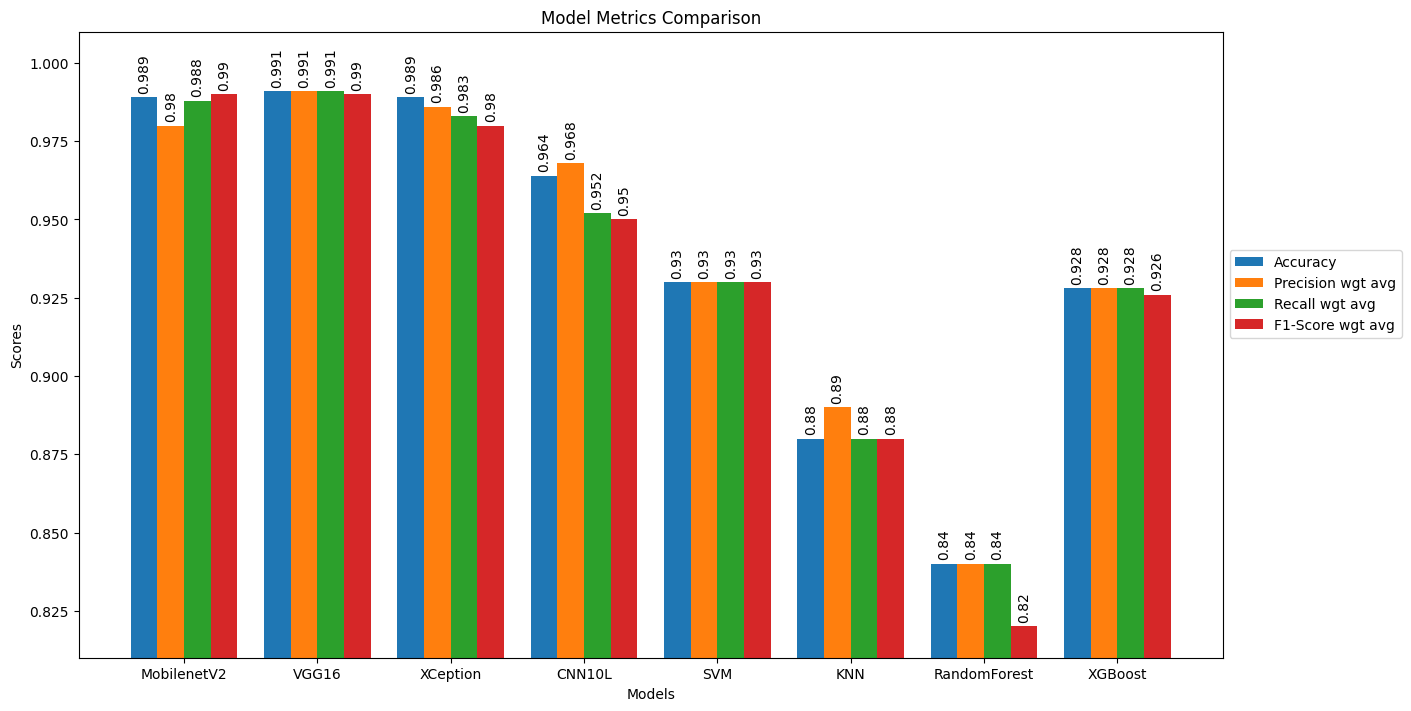
\includegraphics[width=1\linewidth]{graphics//chapter6/all model evaluation.png}
    \caption{All Model Evaluation Metrics}
    \label{fig:all-eval0}
\end{figure}


\begin{figure}
    \centering
    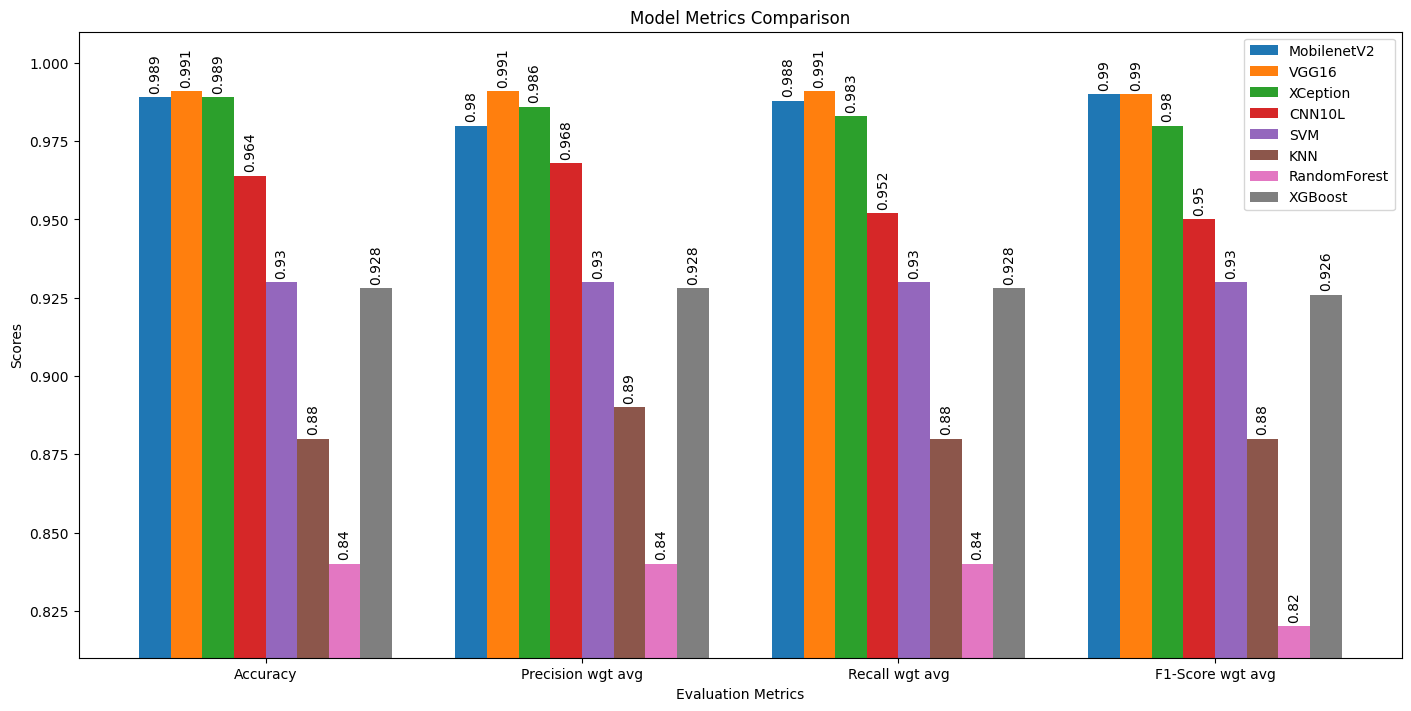
\includegraphics[width=1\linewidth]{graphics//chapter6/model eval grp by metric.png}
    \caption{All Model Evaluation Metrics Group By Metrics Types}
    \label{fig:all-eval1}
\end{figure}

% \FloatBarrier

\subsection{Confusion Matrix Produced by Models on Testing Datasets}

\subsubsection{MobileNetV2 Base Model}

\begin{figure}
    \centering
    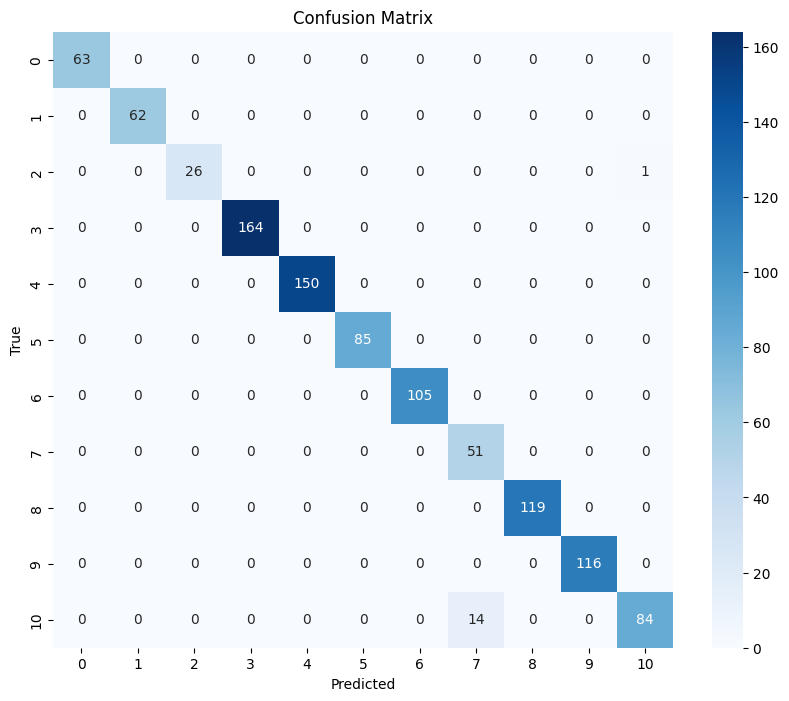
\includegraphics[width=1\linewidth]{graphics//chapter6/cm mobilenetv2.png}
    \caption{Confusion Matrix of MobileNetV2}
    \label{fig:cm-mobnet}
\end{figure}

% \FloatBarrier

\subsubsection{VGG16 Base Model}

\begin{figure}
    \centering
    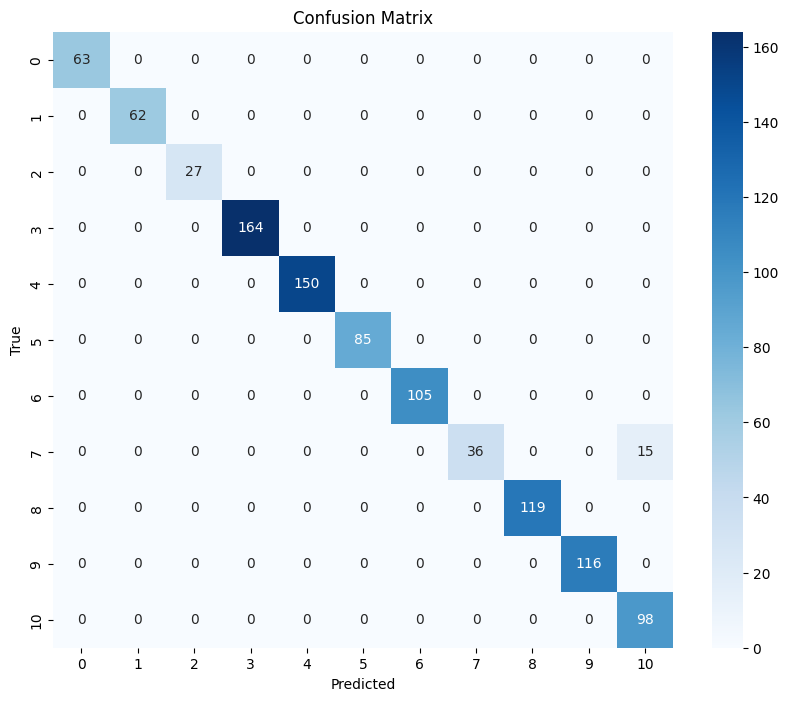
\includegraphics[width=1\linewidth]{graphics//chapter6/cm vgg16.png}
    \caption{Confusion Matrix of VGG16}
    \label{fig:cm-vgg16}
\end{figure}

\subsubsection{Xception Base Model}
\begin{figure}
    \centering
    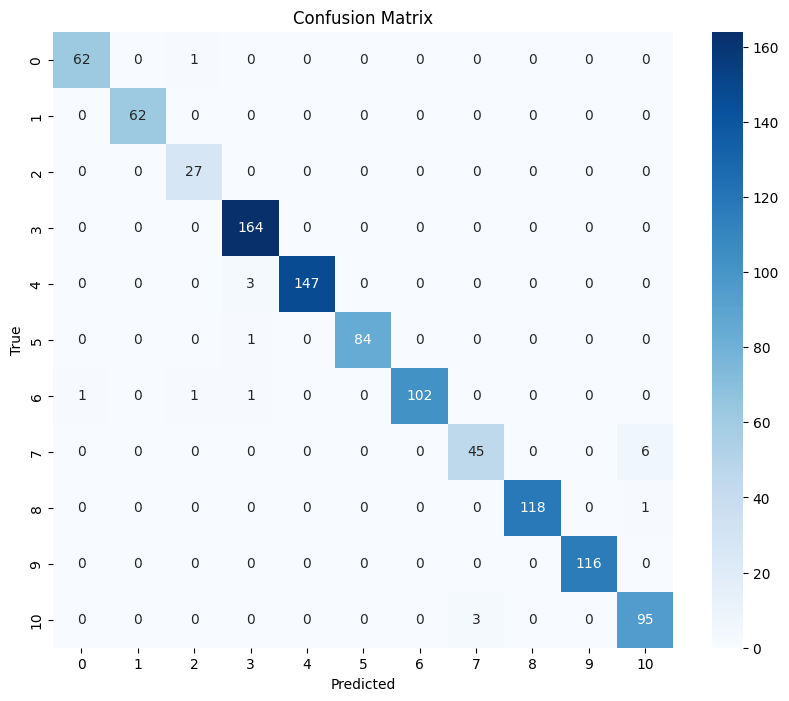
\includegraphics[width=1\linewidth]{graphics//chapter6/cm xception.png}
    \caption{Confusion Matrix of Xception}
    \label{fig:cm-xception}
\end{figure}

\subsubsection{CNN10L Model}
\begin{figure}
    \centering
    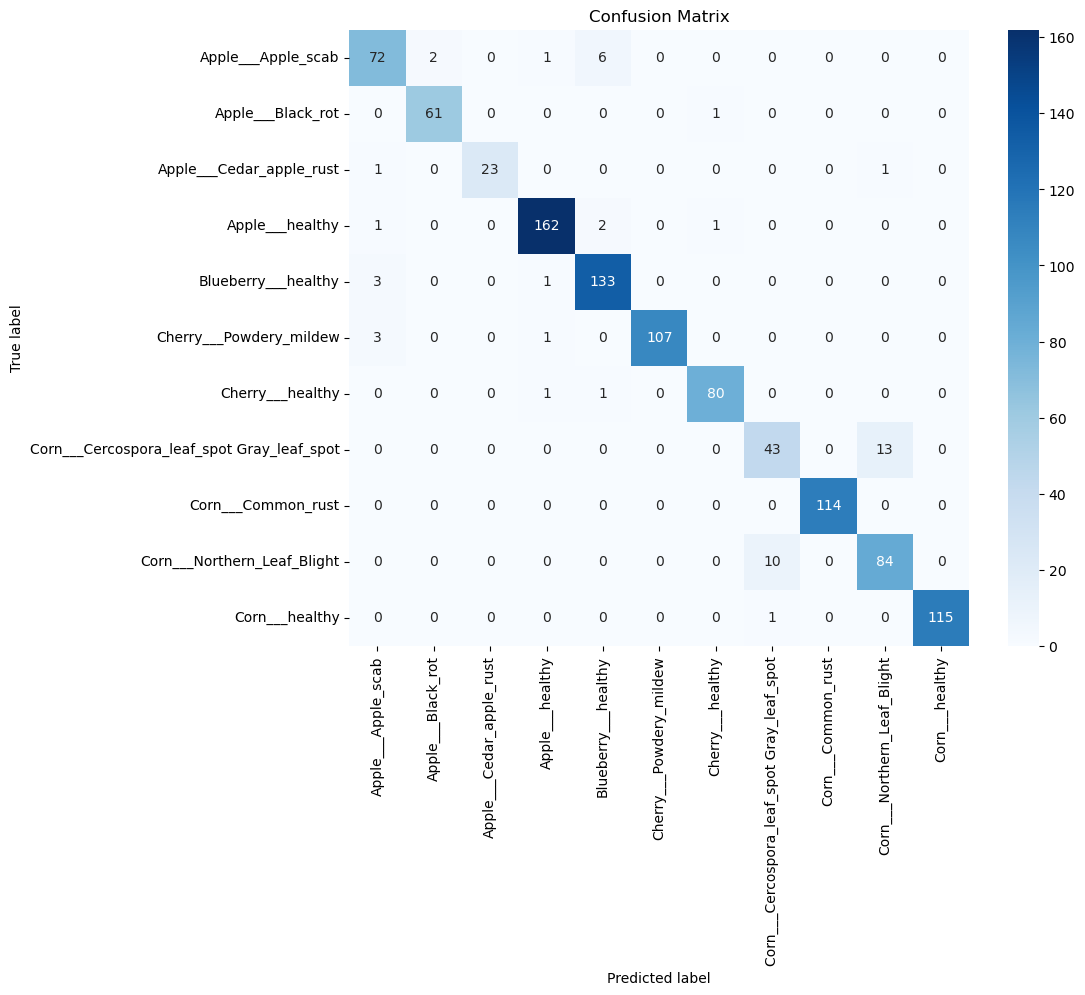
\includegraphics[width=1\linewidth]{graphics/chapter6/cm cnn10l.png}
    \caption{Confusion Matrix of CNN10L Model}
    \label{fig:cm-CNN10L}
\end{figure}



\subsubsection{MobileNetV2 + SVM Model}

\begin{figure}
    \centering
    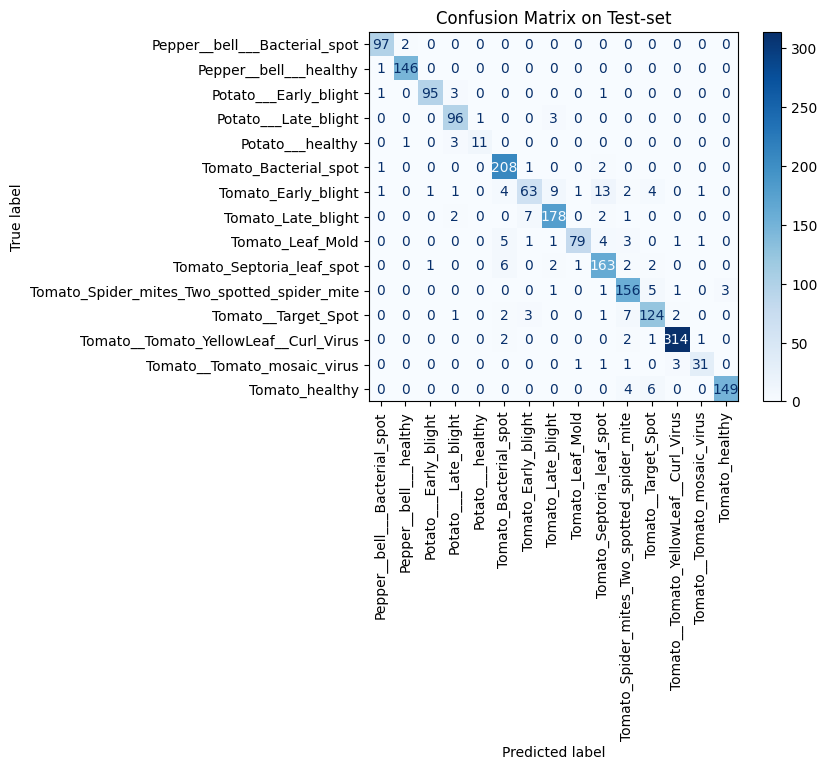
\includegraphics[width=1\linewidth]{graphics//chapter6/cm SVM.png}
    \caption{Confusion Matrix of MobileNetV2 + SVM Model}
    \label{fig:cm-svm}
\end{figure}
\subsubsection{MobileNetV2 + KNN Model}
\begin{figure}
    \centering
    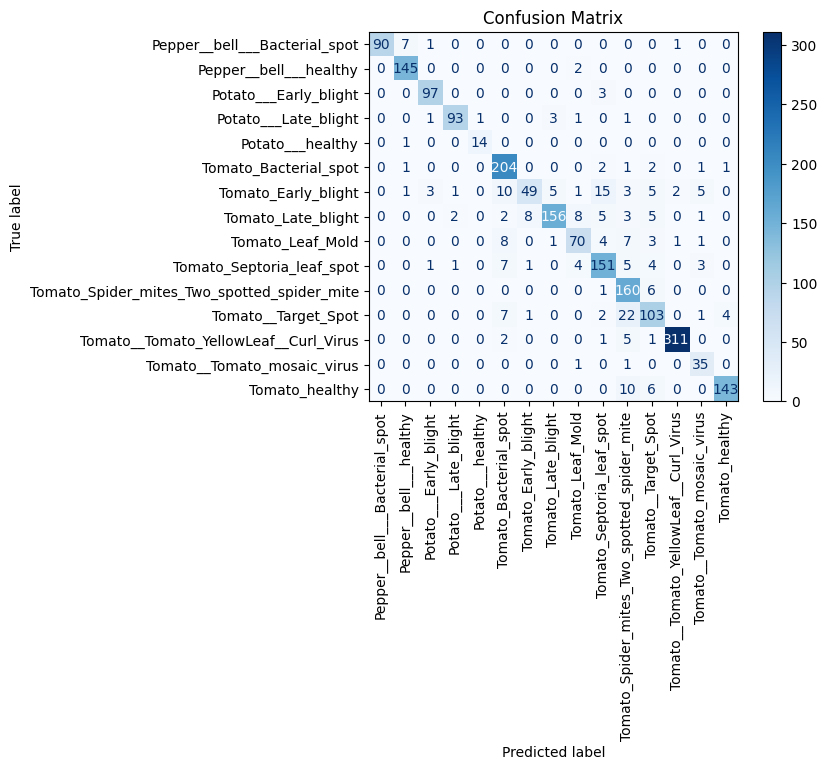
\includegraphics[width=1\linewidth]{graphics//chapter6/cm knn.png}
    \caption{Confusion Matrix of MobileNetV2 + KNN}
    \label{fig:cm-knn}
\end{figure}

\subsubsection{MobileNetV2 + Random Forest Model}
\begin{figure}
    \centering
    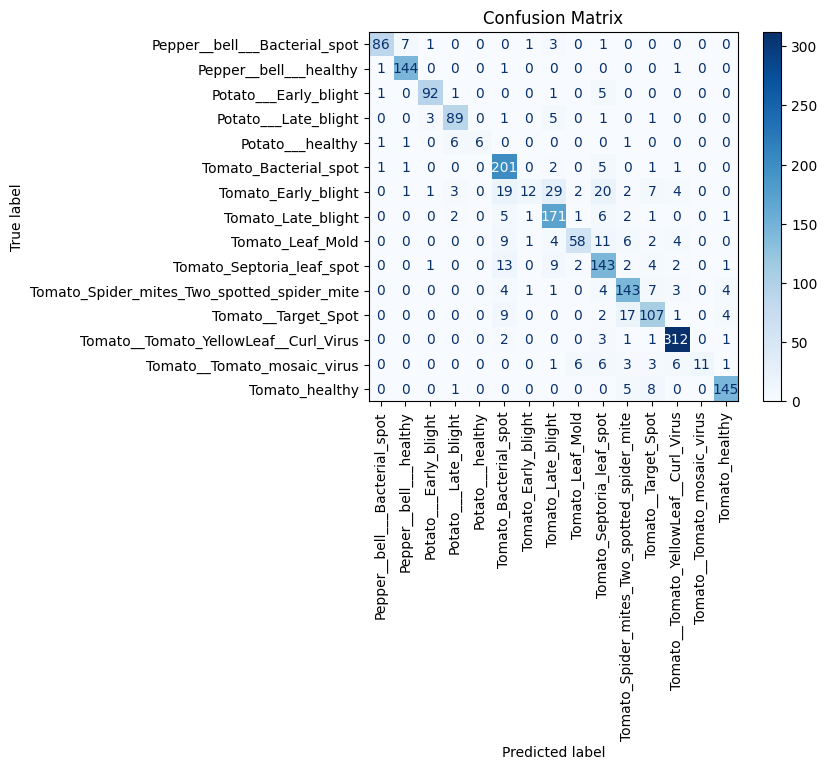
\includegraphics[width=1\linewidth]{graphics//chapter6/cm random forest.png}
    \caption{Confusion Matrix of MobileNetV2 + Random Forest}
    \label{fig:cm-xgboost}
\end{figure}

\subsubsection{MobileNetV2 + XGBoost Model}

\begin{figure}
    \centering
    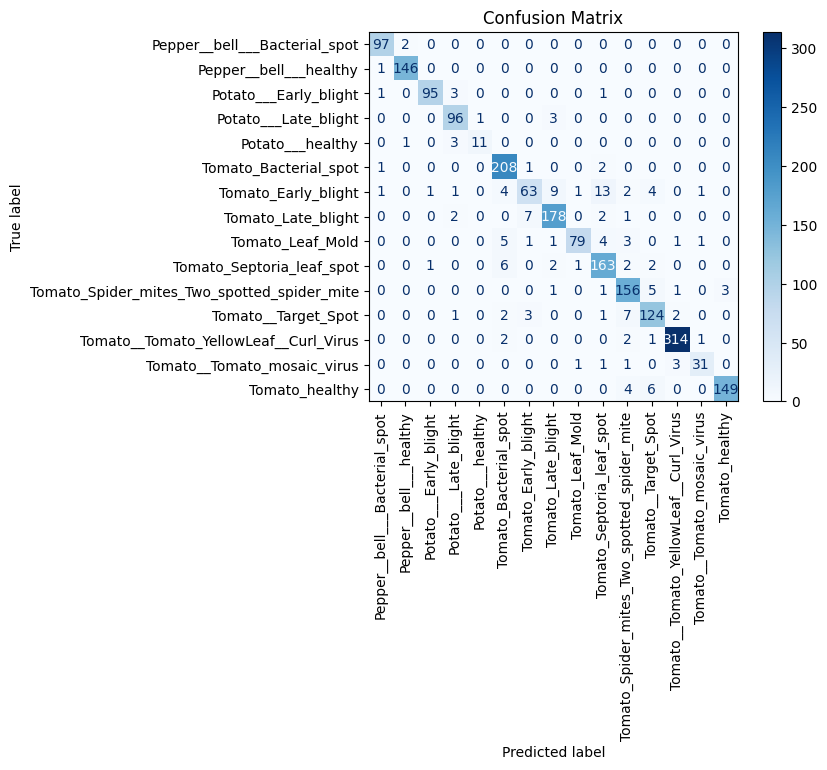
\includegraphics[width=1\linewidth]{graphics//chapter6/cm xgboost.png}
    \caption{Confusion Matrix of MobileNetV2 + XGBoost}
    \label{fig:cm-xgboost}
\end{figure}

% \FloatBarrier
\subsection{Model Prediction}

\begin{figure}
    \centering
    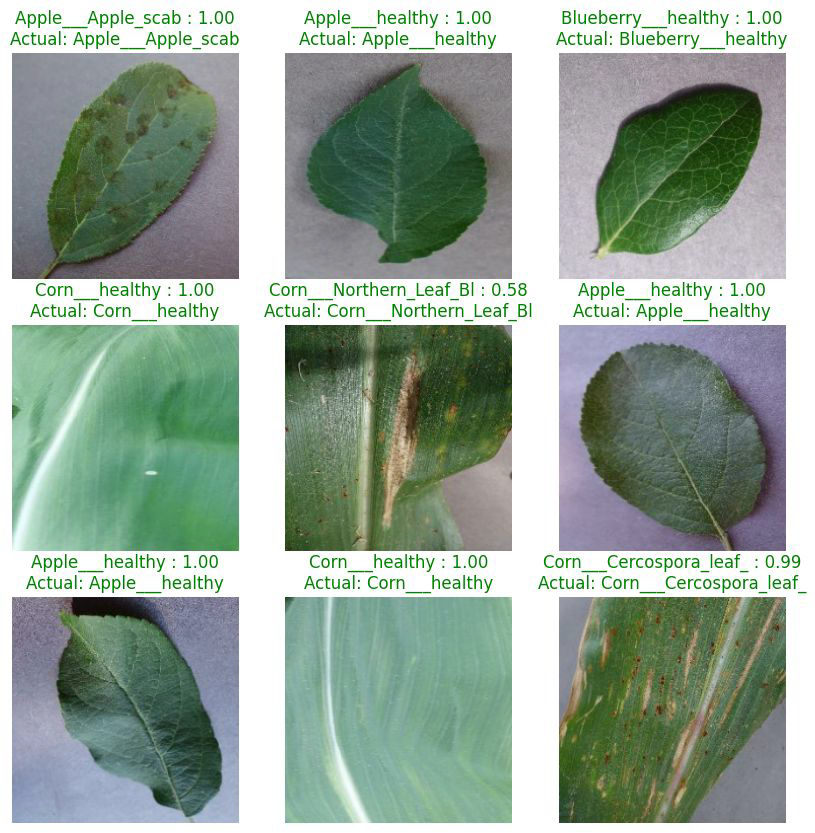
\includegraphics[width=1\linewidth]{graphics//chapter6/vgg prediction0.png}
    \caption{VGG16 Model Prediction}
    \label{fig:vgg-prediction0}
\end{figure}

\begin{figure}
    \centering
    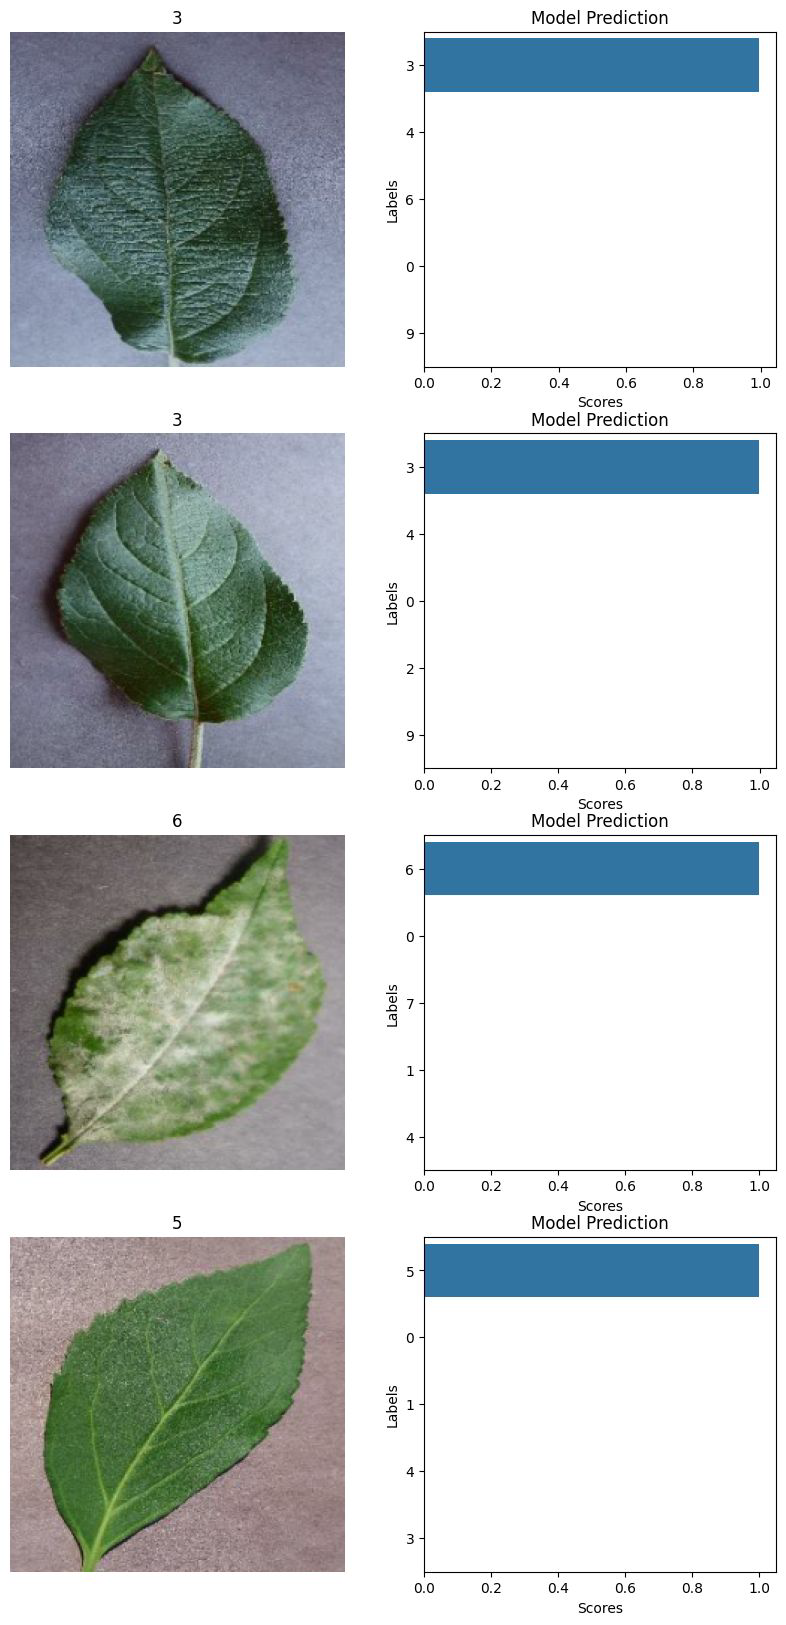
\includegraphics[height=\textheight]{graphics//chapter6/model prediction1.png}
    \caption{VGG-16 Model Prediction - Sample1}
    \label{fig:vgg-prediction1}
\end{figure}

\FloatBarrier